

%_________________________________________________________________________________
\chapter{Mountain grasslands}
Message here ?
\section{Photograph of mountain grasslands}

\section{Mountain grasslands, source of services}

\section{Mountain grasslands under climate change}

%_________________________________________________________________________________
\chapter{Modelling ecological systems}
Message here ?
\section{Models as understanding and testing tools}

\begin{quote}
"Physicien de la biologie"
\end{quote}
Justify the modelling approach - what's a model ? simplification of reality\\
Long subject refer to models in ecosystem sciences. Different classes of model, and different objectives. Mechanistic models: understanding and testing hypothesis.\\
Model as understanding tools: how does modelling help us understanding the system we are modelling.\\
The need for mechanistic model and emergent properties of models. Process-based models vs statistical model (what happen outside the data (example of flickering tails of regression models), similar to bayesian approach, the model is constrained by our understanding of processes.) \\

\section{Modelling plant communities}

\subsection{Different levels of modelling}

\subsection{Processes}

\subsection{Agent-based models}


\section{Modelling coexistence}
Message here ?

\subsection{What is diversity?}
\begin{figure}
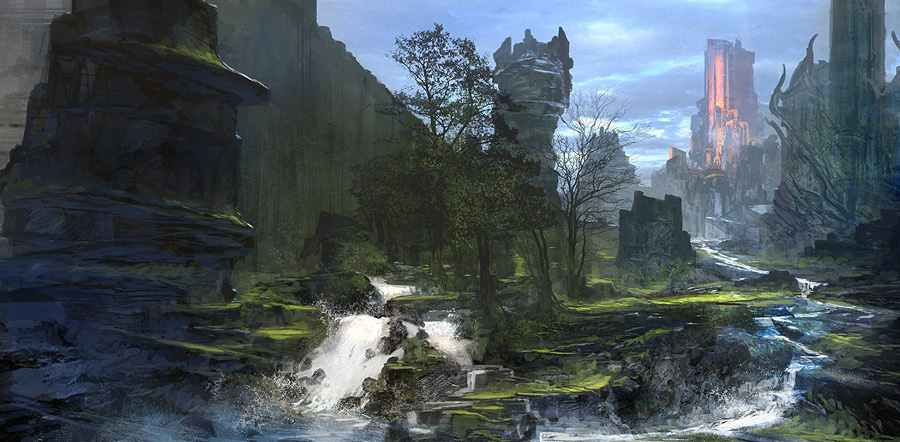
\includegraphics[scale=1]{./Introduction/graphics/plankton.jpg}
\end{figure}

\subsection{The concept of niche}


\subsection{Coexistence mechanisms}

%_________________________________________________________________________________
\chapter{Phenotypic plasticity of organisms}
Message here ?

\section{Stability and plasticity}

\section{Costs and limits of plasticity}

